% MIT License

% Copyright (c) 2022-2023 Melonbob (Robert F. Burgie) <brew.Melonbob@mac.com>

% Permission is hereby granted, free of charge, to any person obtaining a copy
% of this software and associated documentation files (the "Software"), to deal
% in the Software without restriction, including without limitation the rights
% to use, copy, modify, merge, publish, distribute, sublicense, and/or sell
% copies of the Software, and to permit persons to whom the Software is
% furnished to do so, subject to the following conditions:

% The above copyright notice and this permission notice shall be included in all
% copies or substantial portions of the Software.

% THE SOFTWARE IS PROVIDED "AS IS", WITHOUT WARRANTY OF ANY KIND, EXPRESS OR
% IMPLIED, INCLUDING BUT NOT LIMITED TO THE WARRANTIES OF MERCHANTABILITY,
% FITNESS FOR A PARTICULAR PURPOSE AND NONINFRINGEMENT. IN NO EVENT SHALL THE
% AUTHORS OR COPYRIGHT HOLDERS BE LIABLE FOR ANY CLAIM, DAMAGES OR OTHER
% LIABILITY, WHETHER IN AN ACTION OF CONTRACT, TORT OR OTHERWISE, ARISING FROM,
% OUT OF OR IN CONNECTION WITH THE SOFTWARE OR THE USE OR OTHER DEALINGS IN THE
% SOFTWARE.
\documentclass{article}
\usepackage[letterpaper,portrait]{geometry}
\pagenumbering{gobble}
\usepackage{pgfplots,textcomp}
\pgfplotsset{width=12cm,compat=1.15}
\begin{document}
% 4-step: proteinMC rest mash-in; 2INF-modRIMS beta rest; 3INF-modRIMS alpha rest; 4DEC-modRIMS mash-out
% p-I-TR-I-TR-D-TR
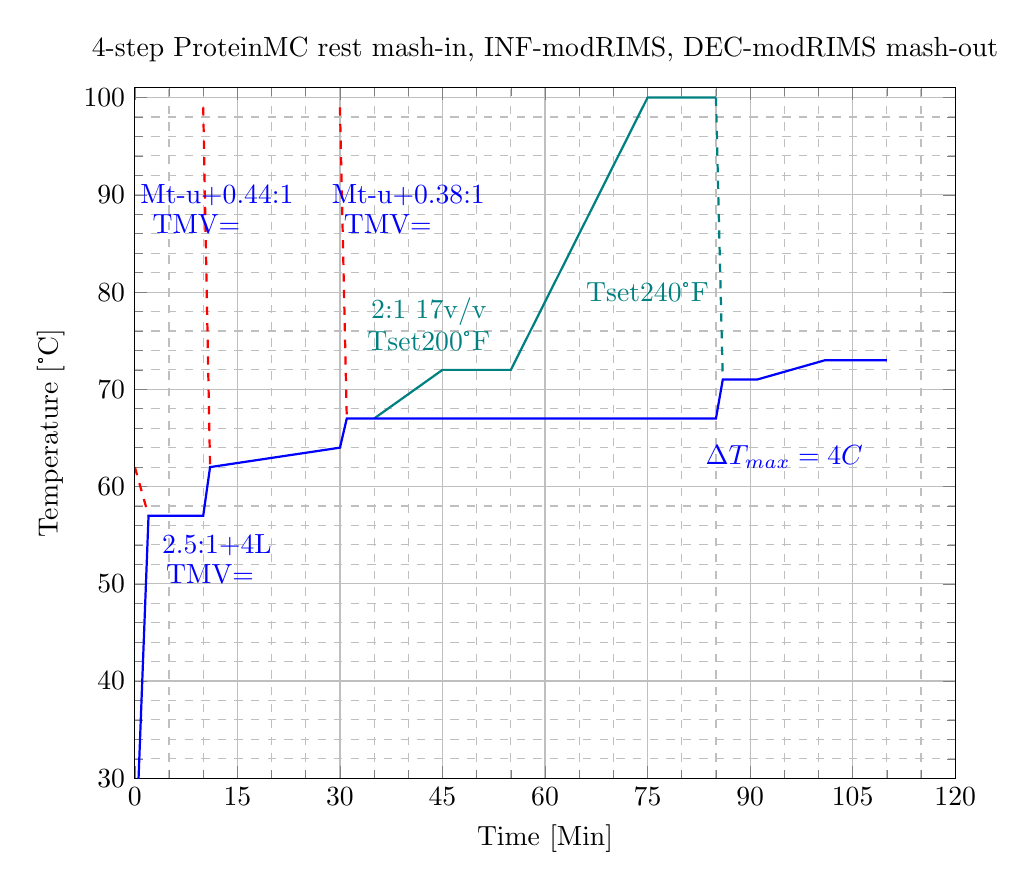
\begin{tikzpicture}
\begin{axis}[
  title={4-step ProteinMC rest mash-in, INF-modRIMS, DEC-modRIMS mash-out},
  xlabel={Time [Min]},
  ylabel={Temperature [\textdegree{C}]},
  xmin=0, xmax=120,
  ymin=30, ymax=101,
  xtick={0,15,30,45,60,75,90,105,120},
  ytick={30,40,50,60,70,80,90,100},
  % legend pos=north west,
  ymajorgrids=true,
  xmajorgrids=true,
  grid style=thin,
  %grid=major,
  minor grid style=dashed,
  yminorgrids=true,
  xminorgrids=true,
  yminorticks=true,
  xminorticks=true,
  minor y tick num=4,
  minor x tick num=2
]
\addplot [color=red, style=dashed,thick]
  coordinates {
    (0,62)% strike temp
    (2,57)% mash-in 2.5:1 (40+4L on PR1 w/ 16kg) TMV=44+0.67*16=55L
  };
\node [color=blue] at (axis cs:12,54) {2.5:1+4L};
\node [color=blue] at (axis cs:11,51) {TMV=   };
\addplot [color=red, style=dashed,thick]
  coordinates {
    (10,99)(11,62)%1INF 0.44:1 (7L on PR1 w/ 16kg) TMV=62L
  };
\node [color=blue] at (axis cs:12,90) {Mt-u+0.44:1 };
\node [color=blue] at (axis cs:9,87) {TMV=   };
\addplot [color=red, style=dashed,thick]
  coordinates {
    (30,99)(31,67)%2INF 0.38:1 (6L on PR1 w/ 16kg) TMV=68L
  };
\node [color=blue] at (axis cs:40,90) {Mt-u+0.38:1 };
\node [color=blue] at (axis cs:37,87) {TMV=   };
\addplot [color=teal, style=thick]
  coordinates {
    (35,67)% 3DEC heat 12L thick (2:1 17v/v)
    (45,72)% 1C/2min (induction set 200F) then
    (55,72) % 10' decoction rest until starch neg
    (75,100)% 3DEC 1.5C/min (induction set 240F)
    (85,100)% boil 10 min
  };
\node [color=teal] at (axis cs:43,78) {2:1 17v/v};
\node [color=teal] at (axis cs:43,75) {Tset200\textdegree{F}};
\node [color=teal] at (axis cs:75,80) {Tset240\textdegree{F}};
\addplot [color=teal, style=dashed,thick]
  coordinates {
    (85,100)(86,71)% recombine
  };
\node [color=blue] at (axis cs:95,63) {$ \Delta T_{max}=4C $};
\addplot [color=blue, style=thick]
  coordinates {
    (0,20)% initial grist temp
    (2,57)% mash-in
    (10,57)% 10' proteinMC rest, no loss with RIMS, w/o cooling loss -4C/hr=-1C/15min
    (11,62)% 1INF 0.44:1 7L on PR1
    (30,64) % 20' beta rest, TmodRIMS 1C/10min
    (31,67) % 2INF 0.38:1 6L on PR1
    (35,67)% 5' alpha rest, no cooling loss w/ RIMS, DEC pulled
    (85,67)% 50' no cooling loss w/ RIMS
    (86,71)% 3DEC recombined 
    (91,71)% 5' dextrin TmodRIMS until starch negative
    (101,73)% TmodRIMS 1C/5min mash-out
    (105,73)% 5' Lauter/ mash bed settle/ no RIMS
    (110,73)% 5' Vorlauf/ no hose
  };
%\legend{p-I-TR-I-D-TR}
 
\end{axis}
\end{tikzpicture}
\end{document}